%%%%%%%%%%%%%%%%%%%%%%%%%%%%%%%%%%%%%%%%%%%%%%%%%%%%%%%%%%%%%%%%%%%%%
% Use the koma-script document style
\documentclass{scrbook}
%\KOMAoptions{twoside=false} % disable two-side formatting for scrbook
% alternatively, for shorter essay, use the following
% \documentclass{scrartcl}
%%%%%%%%%%%%%%%%%%%%%%%%%%%%%%%%%%%%%%%%%%%%%%%%%%%%%%%%%%%%%%%%%%%%%

%%%%%%%%%%%%%%%%%%%%%%%%%%%%%%%%%%%%%%%%%%%%%%%%%%%%%%%%%%%%%%%%%%%%%
% Useful packages
\usepackage{mathtools}
\usepackage{amssymb,bm,bbold}
\usepackage{enumerate}

\usepackage{hhline}
\usepackage{float}

% CSCI-265
\usepackage{tikz}
\usetikzlibrary{automata, positioning, arrows, arrows.meta}


%=================================
% pre-defined theorem environments
\usepackage{amsthm}
\newtheorem{theorem}{Theorem}
\newtheorem{lemma}{Lemma}
\newtheorem{proposition}{Proposition}
\newtheorem{corollary}{Corollary}
\newtheorem{definition}{Definition}
\newtheorem*{remark}{Remark}
\newtheorem*{assumption}{Assumption}

%=================================
% useful commands
\DeclareMathOperator*{\argmin}{arg\,min}
\DeclareMathOperator*{\argmax}{arg\,max}
\DeclareMathOperator*{\supp}{supp}

\def\vec#1{{\ensuremath{\bm{{#1}}}}}
\def\mat#1{\vec{#1}}

%=================================
% convenient notations
\newcommand{\XX}{\mathbb{X}}
\newcommand{\RR}{\mathbb{R}}
\newcommand{\NN}{\mathbb{N}}
\newcommand{\QQ}{\mathbb{Q}}
\newcommand{\ZZ}{\mathbb{Z}}
\newcommand{\EE}{\mathbb{E}}
\newcommand{\PP}{\mathbb{P}}

\newcommand{\sL}{\mathcal{L}}
\newcommand{\sX}{\mathcal{X}}
\newcommand{\sY}{\mathcal{Y}}

\newcommand{\ind}{\mathbb{1}}

\newcommand{\kleene}{{}^\ast}

%%%%%%%%%%%%%%%%%%%%%%%%%%%%%%%%%%%%%%%%%%%%%%%%%%%%%%%%%%%%%%%%%%%%%
% Typography, change document font
\usepackage[tt=false, type1=true]{libertine}
\usepackage[varqu]{zi4}
\usepackage[libertine]{newtxmath}
\usepackage[T1]{fontenc}

\usepackage[protrusion=true,expansion=true]{microtype}

\author{Guy Matz}

\begin{document}
	
\tikzset{
	->, % makes the edges directed 
%		>='stealth', % makes the arrow heads bold 
	node distance=3cm, % specifies the minimum distance between two nodes. Change if necessary. 
	every state/.style={thick, fill=gray!10}, % sets the properties for each ’state’ node 
	initial text=$ $, % sets the text that appears on the start arrow 
}
	
\title{Title}
% \maketitle

% \tableofcontents
% 
% %\bibliography{bibfile}
% 
% \end{document}


\begin{enumerate}

\item \textbf{Concisely describe (in English) the languages accepted by the following DFAs:}

\begin{enumerate}
    \item Words ending in two or more $a$'s or $b$'s

  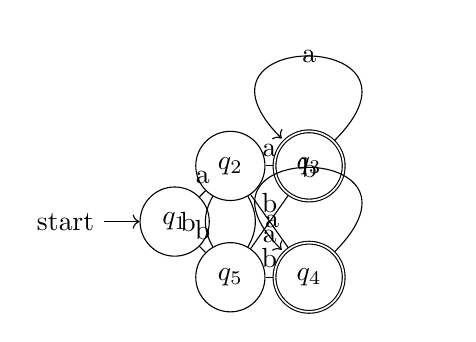
\begin{tikzpicture}
      \node[state, initial] (q1) {$q_1$};
      \node[state, above right of=q1] (q2) {$q_2$};
      \node[state, below right of=q1] (q5) {$q_5$};
      \node[state, accepting, right of=q2] (q3) {$q_3$};
      \node[state, accepting, right of=q5] (q4) {$q_4$};
      \draw
      (q1) edge[above] node{a} (q2)
      (q1) edge[above] node{b} (q5)

      (q2) edge[bend right,  left] node{b} (q5)
      (q5) edge[bend right, right] node{a} (q2)

      (q2) edge[above] node{a} (q3)
      (q5) edge[above] node{b} (q4)

      (q3) edge[above] node{b} (q5)
      (q4) edge[below] node{a} (q2)

      (q3) edge[loop] node{a} (q3)
      (q4) edge[loop] node{b} (q4)
      ;
  \end{tikzpicture}
    \item Odd number of $aaa*$

  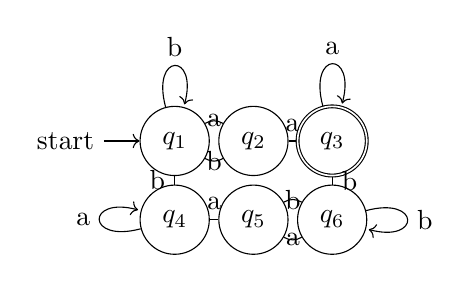
\begin{tikzpicture}
      \node[state, initial] (q1) {$q_1$};
      \node[state, right of=q1] (q2) {$q_2$};
      \node[state, accepting, right of=q2] (q3) {$q_3$};
      \node[state, below of=q1] (q4) {$q_4$};
      \node[state, right of=q4] (q5) {$q_5$};
      \node[state, right of=q5] (q6) {$q_6$};
      \draw
      (q1) edge[loop above] node{b} (q1)
      (q1) edge[bend left] node{a} (q2)
      (q2) edge[bend left] node{b} (q1)
      (q2) edge[above] node{a} (q3)
      (q3) edge[loop above] node{a} (q3)
      (q3) edge[right] node{b} (q6)
      (q6) edge[bend left] node{a} (q5)
      (q5) edge[bend left] node{b} (q6)
      (q5) edge[above] node{a} (q4)
      (q6) edge[loop right] node{b} (q6)
      (q4) edge[loop left] node{a} (q4)
      (q4) edge[left] node{b} (q1)
      ;
  \end{tikzpicture}
\end{enumerate}


\item \textbf{Minimize the following DFAs:}

\begin{enumerate}
    \item

  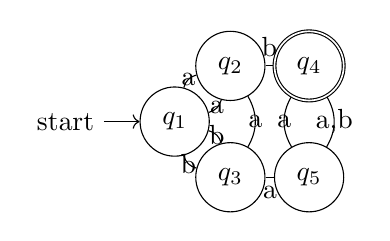
\begin{tikzpicture}
      \node[state, initial] (q1) {$q_1$};
      \node[state, above right of=q1] (q2) {$q_2$};
      \node[state, below right of=q1] (q3) {$q_3$};
      \node[state, accepting, right of=q2] (q4) {$q_4$};
      \node[state, right of=q3] (q5) {$q_5$};
      \draw
      (q1) edge[bend left] node{a} (q2)
      (q2) edge[bend left] node{a} (q1)
      (q1) edge[bend left] node{b} (q3)
      (q3) edge[bend left] node{b} (q1)
      (q3) edge[bend right] node{a} (q2)
      
      (q2) edge[above] node{b} (q4)
      (q5) edge[below] node{a} (q3)
      
      (q4) edge[bend left] node{a,b} (q5)
      (q5) edge[bend left] node{a} (q4)
      
      ;
  \end{tikzpicture}

\begin{table}[]
	\begin{tabular}{|c|c|c|c|c|c}
		\hline
		&  5 &  4 & 3  &   2 \\ \hline
		1 &  &  &  \\ 
		2  &  &  &  \\ \hline
		3  &  &  &  \\ \hline
		4  &  &  &  \\ \hline
	\end{tabular}
\end{table}

    \item

  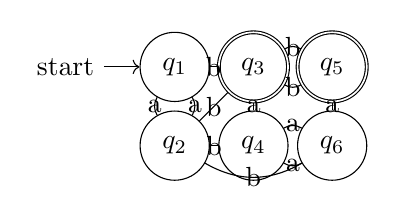
\begin{tikzpicture}
    \node[state, initial] (q1) {$q_1$};
	\node[state, below of=q1] (q2) {$q_2$};
	\node[state, accepting, right of=q1] (q3) {$q_3$};
	\node[state, right of=q2] (q4) {$q_4$};
	\node[state, accepting, right of=q3] (q5) {$q_5$};
	\node[state, below of=q5] (q6) {$q_6$};
	\draw
	(q1) edge[] node{b} (q3)
	(q3) edge[bend left] node{b} (q5)
	(q5) edge[bend left] node{b} (q3)
	
	(q5) edge[] node{a} (q6)

(q6) edge[bend left] node{a} (q4)
(q4) edge[bend left] node{a} (q6)
(q6) edge[bend left] node{b} (q2)

(q3) edge[] node{a} (q4)
(q4) edge[] node{b} (q2)

(q2) edge[] node{b} (q3)

	(q2) edge[bend left] node{a} (q1)
	(q1) edge[bend left] node{a} (q2)
      ;
  \end{tikzpicture}

\begin{table}[]
	\begin{tabular}{|c|c|c|c|c|c|c}
		\hline
		&  6 & 5 &  4 & 3  &   2 \\ \hline
		1 &  &  &  &  \\ \hline
		2  &  &  &  & \\ \hline
		3  &  &  &  & \\ \hline
		4  &  &  &  & \\ \hline
        5  &  &  &  & \\ \hline
	\end{tabular}
\end{table}

\end{enumerate}

\newpage
\item \textbf{When dealing with strings, exponents denote repetition. For
  example, $a^2=aa$, $a^3=aaa$, $a^n= n a$'s.  Construct a DFA over
  $\{a,b\}$ that recognizes the language of all words ending in $a^xb^y$,
  where $x$ and $y$ are both odd. (Assume that $a^x$ includes the entire group
  of $a$'s.  For example, $aaaa$ can only be counted as $a^4$, and not as a
  single '$a$' followed by $a^3$). Minimize your DFA or ensure that it's
  already minimal.}
\\\\


\newpage
\item \textbf{Write a regular expression that defines the language over
  $\{a,b,c\}$, consisting of all words that begin and end in a double ‘$c$’, contain at least one letter between the starting double ‘$c$’ and the ending double ‘$c$’, where $b$’s must occur in groups of 2  or more, and each group of $b$’s must be preceded by an ‘$a$’.}
\\\\

\newpage
\item \textbf{Write a regular expression that defines the language over
  ${a,b,c}$, consisting of all words in which $c$'s can only occur when an odd
  number of $a$'s have been seen up to that point. So $c$'s can occur between the 1st and 2nd $a$'s, and between the 3rd and 4th $a$'s, but not between the 2nd and 3rd $a$'s (and so on).}
\\\\


\newpage
\item \textbf{Proofs: provide an argument for each answer. Make it as
  proof-like as you can.}
\begin{enumerate}
  \item For two regular languages $L1$ and $L2$, is $L1L2$ a proper subset of
    $L1$ always, sometimes, or never?
  \item Prove or disprove (true or false): The regular expression $(a+b)*c$
    describes the language consisting of all words which end in "$c$".
\end{enumerate}

\newpage
\item \textbf{Exercise 2.2.6a (p. 54) - Keep in mind that when reading binary
  from left to right, each additional bit multiplies the value of the
  previously seen bits by 2, and then may add 1 or not. Use this to your
  advantage, while keeping track of the number's value mod 5.}
\\\\


\end{enumerate}

% %\bibliography{bibfile}

\end{document}

